\documentclass[a4paper,10pt,BCOR10mm,oneside,headsepline]{scrartcl}
\usepackage{amsmath, mathtools}
\usepackage[ngerman]{babel}
\usepackage[utf8]{inputenc}
\usepackage{graphicx}


\usepackage{float}

\usepackage{typearea, url}
\areaset{17cm}{26cm}
\setlength{\topmargin}{-1cm}
\usepackage{scrlayer-scrpage}
\pagestyle{scrheadings}

\usepackage[T1]{fontenc}
\usepackage{beramono}
\usepackage{listings}
\usepackage[usenames,dvipsnames]{xcolor}


%%
%% Julia definition (c) 2014 Jubobs
%%
\lstdefinelanguage{Julia}%
  {morekeywords={abstract,break,case,catch,const,continue,do,else,elseif,%
      end,export,false,for,function,immutable,import,importall,if,in,%
      macro,module,otherwise,quote,return,switch,true,try,type,typealias,%
      using,while},%
   sensitive=true,%
   alsoother={$},%
   morecomment=[l]\#,%
   morecomment=[n]{\#=}{=\#},%
   morestring=[s]{"}{"},%
   morestring=[m]{'}{'},%
}[keywords,comments,strings]%

\lstset{%
    language         = Julia,
    basicstyle       = \ttfamily,
    keywordstyle     = \bfseries\color{blue},
    stringstyle      = \color{magenta},
    commentstyle     = \color{ForestGreen},
    showstringspaces = false,
}



\ihead{HW1: CIS 410/510, Computational Science, Fall 2022}
\ohead{\pagemark}
\chead{}
\cfoot{}

%%%%%%%%%%%%%%%%%%%%%%%%%%%%%%%%%%%%%%%%%%%%%%%%%%%%%%%%%%%%
%% Beginning of questionnaire command definitions %%
%%%%%%%%%%%%%%%%%%%%%%%%%%%%%%%%%%%%%%%%%%%%%%%%%%%%%%%%%%%%
%%
%% 2010, 2012 by Sven Hartenstein
%% mail@svenhartenstein.de
%% http://www.svenhartenstein.de
%%
%% Please be warned that this is NOT a full-featured framework for
%% creating (all sorts of) questionnaires. Rather, it is a small
%% collection of LaTeX commands that I found useful when creating a
%% questionnaire. Feel free to copy and adjust any parts you like.
%% Most probably, you will want to change the commands, so that they
%% fit your taste.
%%
%% Also note that I am not a LaTeX expert! Things can very likely be
%% done much more elegant than I was able to. If you have suggestions
%% about what can be improved please send me an email. I intend to
%% add good tipps to my website and to name contributers of course.
%%
%% 10/2012: Thanks to karathan for the suggestion to put \noindent
%% before \rule!

%% \Qq = Questionaire question. Oh, this is just too simple. It helps
%% making it easy to globally change the appearance of questions.
\newcommand{\Qq}[1]{\textbf{#1}}

%% \QO = Circle or box to be ticked. Used both by direct call and by
%% \Qrating and \Qlist.
\newcommand{\QO}{$\Box$}% or: $\ocircle$

%% \Qrating = Automatically create a rating scale with NUM steps, like
%% this: 0--0--0--0--0.
\newcounter{qr}
\newcommand{\Qrating}[1]{\QO\forloop{qr}{1}{\value{qr} < #1}{---\QO}}

%% \Qline = Again, this is very simple. It helps setting the line
%% thickness globally. Used both by direct call and by \Qlines.
\newcommand{\Qline}[1]{\noindent\rule{#1}{0.6pt}}

%% \Qlines = Insert NUM lines with width=\linewith. You can change the
%% \vskip value to adjust the spacing.
\newcounter{ql}
\newcommand{\Qlines}[1]{\forloop{ql}{0}{\value{ql}<#1}{\vskip0em\Qline{\linewidth}}}

%% \Qlist = This is an environment very similar to itemize but with
%% \QO in front of each list item. Useful for classical multiple
%% choice. Change leftmargin and topsep accourding to your taste.
\newenvironment{Qlist}{%
\renewcommand{\labelitemi}{\QO}
\begin{itemize}[leftmargin=1.5em,topsep=-.5em]
}{%
\end{itemize}
}

%% \Qtab = A "tabulator simulation". The first argument is the
%% distance from the left margin. The second argument is content which
%% is indented within the current row.
\newlength{\qt}
\newcommand{\Qtab}[2]{
\setlength{\qt}{\linewidth}
\addtolength{\qt}{-#1}
\hfill\parbox[t]{\qt}{\raggedright #2}
}

%% \Qitem = Item with automatic numbering. The first optional argument
%% can be used to create sub-items like 2a, 2b, 2c, ... The item
%% number is increased if the first argument is omitted or equals 'a'.
%% You will have to adjust this if you prefer a different numbering
%% scheme. Adjust topsep and leftmargin as needed.
\newcounter{itemnummer}
\newcommand{\Qitem}[2][]{% #1 optional, #2 notwendig
\ifthenelse{\equal{#1}{}}{\stepcounter{itemnummer}}{}
\ifthenelse{\equal{#1}{a}}{\stepcounter{itemnummer}}{}
\begin{enumerate}[topsep=2pt,leftmargin=2.8em]
\item[\textbf{\arabic{itemnummer}#1.}] #2
\end{enumerate}
}

%% \QItem = Like \Qitem but with alternating background color. This
%% might be error prone as I hard-coded some lengths (-5.25pt and
%% -3pt)! I do not yet understand why I need them.
\definecolor{bgodd}{rgb}{0.8,0.8,0.8}
\definecolor{bgeven}{rgb}{0.9,0.9,0.9}
\newcounter{itemoddeven}
\newlength{\gb}
\newcommand{\QItem}[2][]{% #1 optional, #2 notwendig
\setlength{\gb}{\linewidth}
\addtolength{\gb}{-5.25pt}
\ifthenelse{\equal{\value{itemoddeven}}{0}}{%
\noindent\colorbox{bgeven}{\hskip-3pt\begin{minipage}{\gb}\Qitem[#1]{#2}\end{minipage}}%
\stepcounter{itemoddeven}%
}{%
\noindent\colorbox{bgodd}{\hskip-3pt\begin{minipage}{\gb}\Qitem[#1]{#2}\end{minipage}}%
\setcounter{itemoddeven}{0}%
}
}

%%%%%%%%%%%%%%%%%%%%%%%%%%%%%%%%%%%%%%%%%%%%%%%%%%%%%%%%%%%%
%% End of questionnaire command definitions %%
%%%%%%%%%%%%%%%%%%%%%%%%%%%%%%%%%%%%%%%%%%%%%%%%%%%%%%%%%%%%

\begin{document}

\begin{center}
\textbf{\large CIS 410/510 HW 4 - Brett Sumser%\footnote{Subject to change}
}
\end{center}\vskip1em


\begin{figure}[h]
\centering
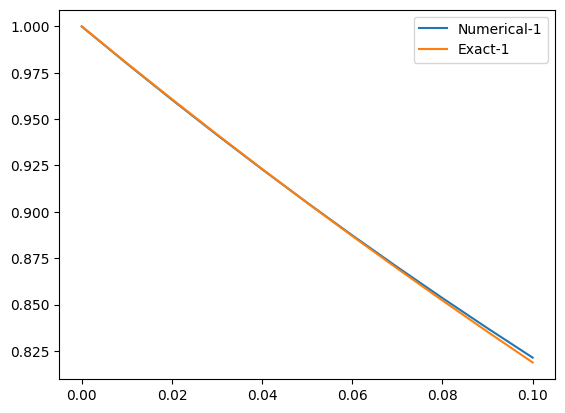
\includegraphics[scale=0.4]{fig1.png}
\end{figure}


\newpage

\begin{lstlisting}

using LinearAlgebra
using Plots
using Printf # for formatting text output

"""
    var_set(N)

Initializes banded sparse matrix, and vector b of size N


A = -2 1 0 .... 0
     0-2 1 0 .. 0
     0 0-2 1 0  0
"""
function var_set(N)
    A = Matrix{Float64}(undef, N, N)
    A = zeros(N,N)

    A_d = Matrix{Float64}(undef, N, N)
    A_d = ones(N,N)
    for i = 1:N
        A_d[i,i] = -2
    end

    b = rand(N,1)
    b = b[:]

    for i = 1:N
        b[i] = 1
    end

    for i = 1:N
        A[i,i] = -2
        if i != N
            A[i, i+1] = 1
            A[i+1, i] = 1
        end
    end

    return (A, A_d, b)
end


"""
    LU_solve(A, b)

Uses Julia linear algebra package to solve Ax = b
given Matrix A and vector b
"""
function LU_solve(A, b)
    F = lu(A)
    # display(F)

    x = F\b

    # display(x)
    return x
end

function main()
    dense_time = []
    sparse_time = []
    testSizes = [10, 100, 1000, 10000]
    @printf("starting loop for values")
    for i = 1:size(testSizes,1)
        (A, A_d, b) = var_set(testSizes[i])
        temp = @timed x = LU_solve(A, b)
        push!(sparse_time, temp[2])
        new_temp = @timed x = LU_solve(A_d, b)
        push!(dense_time, new_temp[2])
        @printf("done at N = %d\n", testSizes[i])
    end
    scatter(testSizes, dense_time, color="red", xlabel="Size of N", ylabel="Time", title = "Size of N vs Time", legend=false)
    scatter!(testSizes, sparse_time, color="blue", legend=false)
    savefig("denseSparsePlot.png")
end

main()



using LinearAlgebra
using Plots
using Printf # for formatting text output

"""
    var_set(N)

Initializes banded sparse matrix, and vector b of size N


A = -2 1 0 .... 0
     0-2 1 0 .. 0
     0 0-2 1 0  0
"""
function var_set(N)
    A = Matrix{Float64}(undef, N, N)
    A = zeros(N,N)

    A_d = Matrix{Float64}(undef, N, N)
    A_d = ones(N,N)
    for i = 1:N
        A_d[i,i] = -2
    end

    b = rand(N,1)
    b = b[:]

    for i = 1:N
        b[i] = 1
    end

    for i = 1:N
        A[i,i] = -2
        if i != N
            A[i, i+1] = 1
            A[i+1, i] = 1
        end
    end

    return (A, A_d, b)
end


"""
    LU_solve(A, b)

Uses Julia linear algebra package to solve Ax = b
given Matrix A and vector b
"""
function LU_solve(A, b)
    F = lu(A)
    # display(F)

    x = F\b

    # display(x)
    return x
end

function main()
    dense_time = []
    sparse_time = []
    testSizes = [10, 100, 1000, 10000]
    @printf("starting loop for values")
    for i = 1:size(testSizes,1)
        (A, A_d, b) = var_set(testSizes[i])
        temp = @timed x = LU_solve(A, b)
        push!(sparse_time, temp[2])
        new_temp = @timed x = LU_solve(A_d, b)
        push!(dense_time, new_temp[2])
        @printf("done at N = %d\n", testSizes[i])
    end
    scatter(testSizes, dense_time, color="red", xlabel="Size of N", ylabel="Time", title = "Size of N vs Time", legend=false)
    scatter!(testSizes, sparse_time, color="blue", legend=false)
    savefig("denseSparsePlot.png")
end

main()


using Plots

# write forward Euler for the IVP system y' = f(t, y)
# where y is a vector in R^n (i.e. has n components)


function my_forward_euler_linear(t0, Tf, Δt, y0, A, b)

    # y0 has N components
    N = length(y0)
    display(y0)
    show(stdout, N)

    M = Integer(Tf/Δt)  # M+1 total temporal nodes

    t = Vector{Float64}(undef, M+1)
    y = Matrix{Float64}(undef, N, M+1)

    # fill in the initial condition:
    t[1] = t0
    y[:, 1] = y0

    for n = 1:M # take M time steps
        y[:, n+1] = y[:, n] + Δt*(A*y[:, n] + b(t[n]))
        t[n+1] = t[n] + Δt
    end

    return (t, y)
end

function my_forward_euler(t0, Tf, Δt, y0, f)

    # y0 has N components
    N = size(y0)

    M = Integer(Tf/Δt)  # M+1 total temporal nodes

    t = Vector{Float64}(undef, M+1)
    y = Matrix{Float64}(undef, N, M+1)

    # fill in the initial condition:
    t[1] = t0
    y[:, 1] = y0

    for n = 1:M # take N time steps
        y[:, n+1] = y[:, n] + Δt*f(t[n],y[:, n])
        t[n+1] = t[n] + Δt
    end

    return (t, y)
end

function var_set(N)
    A = Matrix{Float64}(undef, N, N)
    A = rand(N,N)

    y = rand(N,1)
    y = y[:]

    for i = 1:N
        y[i] = 0
    end

    return (A, y)
end


#=
# Write forward Euler to solve the linear system IVP:
# y' = Ay + b on 0 ≤ t ≤ Tf
# with initial y0
# Do this on particular example, where A = [-3 13; -5 -1]
# y0 = [3; -10]
t0 = 0
y0 = [3; -10]
A = [-3 13;-5 -1]
Tf = 10
Δt = 1
N = Integer(Tf/Δt) # N+1 total temporal nodes
y = Matrix{Float64}(undef, 2, N+1)
t = Vector{Float64}(undef, N+1)
t[1] = 0
# fill in initial condition:
y[:, 1] = y0
for n = 1:N  # take N time steps
    y[:, n+1] = y[:, n] + Δt*A*y[:, n]  # Forward Euler
    t[n+1] = t[n] + Δt
end
#plot(t, y[1, :])  # plot first component of solution vector
#plot!(t, y[2, :])  # plot second component
# plot initial condition:
p = plot([y[1, 1]], [y[2, 1]], marker=(:circle,5), color = :blue, legend = false)
for n = 2:N+1
    p = plot!([y[1, n]], [y[2, n]], marker=(:circle,5), color = :blue, legend = false)
    display(p)
    sleep(1)
end
=#

\end{lstlisting}
\end{document}
